\documentclass[conference]{IEEEtran}

\usepackage{xspace}
\usepackage{enumitem}
\usepackage{graphicx}
\usepackage{fancyvrb}
\usepackage{amssymb,amsmath,amsthm}
\graphicspath{{graphics/}}
\usepackage{color}
\usepackage{hyperref}           
\usepackage{tabularx}
\usepackage{eucal}
\usepackage{booktabs}

\usepackage{listings}
\lstset{captionpos=b,language=verilog,morekeywords={assert,property}}

\hypersetup{
    colorlinks=true,
    linkcolor=blue,
    citecolor=blue,
    filecolor=red,      
    urlcolor=magenta,
    breaklinks=true,            
}


\newcommand{\cks}[1]{\textcolor{red}{cks: #1}}

\newcommand{\twopartdef}[4]
{
	\left\{
		\begin{array}{ll}
			#1 & \mbox{if } #2 \\
			#3 & \mbox{if } #4
		\end{array}
	\right.
}

%% Text and formatting
\setlist[itemize]{noitemsep, topsep=0pt}
\setlist[enumerate]{noitemsep, topsep=0pt}

\theoremstyle{definition}
\newtheorem{definition}{Definition}
\newtheorem{theorem}{Theorem}[section]
\newtheorem{corollary}{Corollary}[theorem]


\graphicspath{ {./figures/} }

\begin{document}

\title{Survey of Weakly-hard Constraints on Distributed Embedded Control Systems}
\author{
  \IEEEauthorblockN{Martin Meng}
\IEEEauthorblockA{The University of North Carolina at Chapel Hill\\
martinmq@live.unc.edu}
}

\maketitle

% This survey has reviewed recent works related to weakly hard constraints with an emphasis on its application to control systems. Various methods to compute and verify weakly-hard guarantees are studied. We focus on weakly hard model's applications to distributed embedded control systems such that the security and robustness of the systems are enhanced. We also study MIP formulation, an optimization technique common in the community of real-time systems. Lastly, we propose a new approach to leverage the weakly hard model to enhance the robustness of distributed embedded control systems in automated vehicles.

\begin{abstract}
  Weakly hard models have been utilized to optimize the design of real-time distributed embedded control systems. This survey serves as an overview of research topics related to weakly hard models with an emphasis on their applications to control systems. Specifically, this survey proposes an approach to leverage the weakly hard model to enhance the robustness of distributed embedded control systems in automatic vehicles. This survey also summaries various methods to compute weakly hard guarantees, studies the impact of deadline miss on the stability of control systems, introduces cases in which weakly hard models are adopted to improve the security and fault tolerance of systems, and studies Mix Integer Programming problems in the context of real-time distributed systems.
\end{abstract}

\begin{IEEEkeywords}
Distributed Systems, Embedded Systems, Controller Design, Real-time Systems, Weakly Hard Models, Cyber-Physical Systems, Security 
\end{IEEEkeywords}

\section{Introduction}
This is where the introduction will go. \cks{We need a better title.}

\section{Weakly Hard Model} \label{model}

Weakly hard model is a formalized description for systems that can sporadically miss deadlines. Bernat et al.~\cite{bernat2001weakly} proposed four definitions on weakly hard models. 

\begin{definition} \label{def:meetany}
A task $\tau$ \emph{"meets any n in m deadlines"}, if for any sequence of m consecutive jobs of $\tau$, there are at least n jobs that meet the deadline.
\end{definition}

\begin{definition} \label{def:meetrow}
 A task $\tau$ \emph{"meets row n in m deadlines"}, if for any sequence of m consecutive jobs of $\tau$, there are at least a sequence of n consecutive jobs that meet the deadline.
\end{definition}

\begin{definition} \label{def:missany}
 A task $\tau$ \emph{"misses any n in m deadlines"}, if for any sequence of m consecutive jobs of $\tau$, there are at most n deadline misses.
 \end{definition}
 
 \begin{definition} \label{def:missrow}
 A task $\tau$ \emph{"misses row n in m deadlines"}, if for any sequence of m consecutive jobs of $\tau$, there are less than n consecutive deadline misses.
 \end{definition}
 
 These four types of weakly hard models are classified by two metrics. The first metric considers whether the model considers deadlines that are met or missed. The other metric considers whether the missed deadlines or deadlines that are met are required to be consecutive or not. Table~\ref{table:1} shows this two-dimensional classification. 

% Table 1
\begin{table}[h!]
\caption{Classification of weakly hard models}
 \begin{center}
 \begin{tabular}{| c | c c |} 
 \hline
 Metrics & Met deadlines & Missed deadlines\\ [0.5ex] 
 \hline
 Consecutive & Definition~\ref{def:meetrow} & Definition~\ref{def:missrow} \\ 
Any order & Definition~\ref{def:meetany} & Definition~\ref{def:missany} \\ 
 \hline
\end{tabular}
\label{table:1}
\end{center}
 \end{table}

% Def 3 is popular. Def 4 is studied
The research community has focused on the model \emph{"misses any n in m deadlines"} defined in Definition~\ref{def:missany}, also called the m-K model. For example, Frehse et al. used model checking technique to analysis the schedulability under m-K model~\cite{frehse2014formal}. The analysis of Sun et al. on periodic tasks with static priorities with free offsets is based on m-K model as well~\cite{sun2017weakly}. Moreover, designing stable controller on the m-K model has been studied~\cite{linsenmayer2017stabilization}. 

However, m-K model does not have any constraint on the consecutiveness of the deadline misses, but industrial cases often require consideration of the consecutiveness of deadline misses~\cite{maggio2020control}. Therefore, Maggio et al. considered the model in Definition~\ref{def:missrow} which bounds the maximum number of consecutive deadline misses. They analyzed the stability of control systems based on this model by considering joint spectral radius~\cite{maggio2020control}. 

The relationship between the models "misses row n in m deadlines" (Definition~\ref{def:missrow}) and "misses any n in m deadlines" (Definition~\ref{def:missany}, m-K model) is that the model "misses row n in m deadlines" imposes additional constraints about consecutiveness on the task set and thus is a tighter model. Therefore, if a task set is schedulable on the model "misses any n in m deadlines" (Definition~\ref{def:missany}), then the task set is guaranteed to be schedulable on the model "misses row n in m deadlines" (Definition~\ref{def:missrow}). However, there exist cases in which a task set is schedulable on the model "misses row n in m deadlines" (Definition~\ref{def:missrow}) but not on the model "misses any n in m deadlines" (Definition~\ref{def:missany}). For instance, if a task misses n deadlines in a sequence of m consecutive deadlines but the n deadline misses are not consecutive, then this task satisfies the model "misses row n in m deadlines" (Definition~\ref{def:missrow}) but fails to satisfy the model "misses any n in m deadlines" (Definition~\ref{def:missany}). Because the "misses any n in m deadlines" model (Definition~\ref{def:missany}) includes the model "misses row n in m deadlines" (Definition~\ref{def:missrow}) in terms of schedulability, and is more popular in the research community, the rest of this survey will consider the m-K model only.




































\section{Weakly Hard Model and Control Systems} \label{application}

\subsection{Control Systems}
This section studies an example~\cite{liang2019security} to enhance the security and robustness of control systems by leveraging weakly hard constraints. We consider a feedback controller design for physical plants with linear time-invariant model. The dynamics of the system can be formulated by the following state-space model:
\begin{align*}
\dot{x}(t) &= Ax(t) + Bu(t) \\
y(t) &= Cx(t) + Du(t) \\
u(t) &= Ky(t)
\end{align*}
where x(t), y(t), and u(t) are vectors representing the states, the output, and the control input of the system at time t, respectively. A, B, and C are system matrices. 

This continuous model of control systems needs to be discretized before being implementing on digital platforms. We assume that computation delay and communication delay are negligible in the system. A typical model of such discrete system is as follows:
\begin{align*}
    z[k+1] &= A_{aug} z[k] + B_{aug} u[k] \\
    y[k] &= C_{aug} z[k] \\
    u[k] &= -Kz[k]
\end{align*}
where z[k], y[k], and u[k] denote the augmented states, the output, and the control input of the system at time $h_k$, respectively, where $h_k$ denotes the time t at the k-th cycle. K is the feedback gain of the system that ensures the stability of the system. $A_{aug}$  is a matrix $\in$ $\hspace{0.3mm}$ $R^n$ $\times$ $R^n$, $B_{aug}$  is a matrix $\in$$\hspace{0.3mm}$ $R^n$ $\times$ $1$, and $C_{aug}$ is a matrix $\in$ $\hspace{0.3mm}$ $1$ $\times$ $R^n$. 

\subsection{Stability and Control Performance} \label{stability and control performance}
To optimize the design of control systems under the weakly hard model, we need to study the impact of deadline miss pattern on the stability and control performance of the system. A discrete control system as described in the previous section is stable if all the closed-loop poles lie in the unit circle in a complex plane. This system dynamics is described as follows:
\begin{align*}
z[k + 1] &= (A_{aug} - B_{aug}K)z[k] \\
A_{cl} &= A_{aug} - B_{aug}K
\end{align*}
The stability property is formalized as a study of the eigenvalues of the matrix $A_{cl}$. The closed-loop system is stable if and only if all eigenvalues of $A_{cl}$ are within the unit circle in the complex plane, i.e. their lengths are all less than 1.

While stability considers whether the system can be stabilized, control performance measures how quickly the controller can bring the system back to the equilibrium state after a disturbance, assuming the the system can be stabilized. The control performance is quantified by a metric H. H stands for the minimal number of sampling cycles to bring a disturbance J back to a certain predefined threshold $J_{th}$. This property is formalized as the following equation:
\begin{align*}
 \forall r &\ge H \\
 &J_r \le J_th 
\end{align*}

\subsection{Weakly Hard Constraints} \label{weakly hard constraints formulation}
The weakly hard model we take into consideration in this example is the m-K model that allows a task to "misses any n in m deadlines" (Definition~\ref{def:missany}). We quantitively formalize this timing requirement for a task $\tau$ as
\begin{align*}
(k^{j}, N^{j})
\end{align*}
which represents that for a sequence of $N^{j}$ consecutive activations of task $\tau$, there are at most $k^{j}$ deadline misses. 

We also denote
\begin{align*}
dmm(N^j)
\end{align*}
as the number of deadline misses in the worst case for task $\tau$ in any sequence of $N^j$ consecutive activations.

With these notions in hand, we can formally define a task $\tau$ satisfying its weakly hard constraint $(k^{j}, N^{j})$ as follows:
\begin{align*}
dmm(N^j) \le k^j, \forall j
\end{align*}

\subsection{Security Monitoring Tasks}
The goal of this example ~\cite{liang2019security} is to improve the security of the embedded control systems by optimizing the allocation, priority, and period assignments of the security monitoring tasks leveraging the weakly hard constraints. Security monitoring tasks read the CAN messages to detect intrusion. Security monitoring tasks are periodic tasks. For each period, an activation of the security monitoring task reads the CAN messages it monitors and check for anomaly intrusions. Figure ~\ref{fig:system_model} shows a model of system with security monitoring tasks.

\begin{figure}[h!]
\caption{System model with security monitoring tasks~\cite{liang2019security}}
\centering
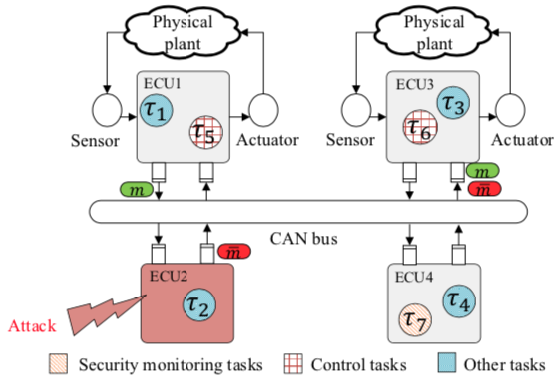
\includegraphics[width=0.5\textwidth]{system_model}
\label{fig:system_model}
\end{figure}

Security monitoring tasks impose constraints on the system design. These constraints are of two types. The first type deals with the coverage of security monitoring tasks. For instance, a constraint asserts that all security critical tasks are monitored by at least one security monitoring task. The second type of constraint is about redundancy. To avoid the single-point failure, a security critical CAN message may require to be monitored by multiple security monitoring tasks on different ECUs. 

\subsection{Optimization Problem}
This example formulates the design problem as a multi-objective optimization problem. The objective of the optimization problem describes the trade-off between control performance and security. The constraints include the stability constraints, control performance constraints, constraints imposed by security monitoring tasks, and schedulability constraints imposed by the weakly hard model.











\section{MIP Formulation} \label{mip}

\subsection{Mix Integer Programming}
Mix Integer Programming (MIP) is a common optimization technique that is widely used by the research community to study weakly hard models. An optimization problem is called an integer programming problem if its decision variables are constrained to integer values. MIP is a special form of integer programming problem in that some variables, but not all, are constrained to be integers. A common type of decision variables in MIP is binary variable whose value is restricted to be 0 or 1, which formulates yes/no question. However, integer programming is NP-Hard because it is not convex, so it takes a large amount of computation time and memory resources to find an optimal solution. In spite of the complexity, industrial solvers can solve small size MIP problem relatively fast. 

\subsection{Ethernet-based Switch Network}
This section considers the application-level scheduling problem on a time-triggered, Ethernet based distributed system ~\cite{Zhang2018SynthesizingCA}. Specifically, a switch network is considered. This network can be model as an undirected graph. The nodes of the graph are end stations and switches that forward messages between end stations. An edge between two nodes represents a full-duplex link that allows simultaneous message transmissions between two nodes. An example of this graph-based presentation of a Ethernet-based switch network is shown in Figure ~\ref{fig:network}.

\begin{figure}[h!]
\caption{A model of Ethernet-based Switch Network~\cite{Zhang2018SynthesizingCA}}
\centering
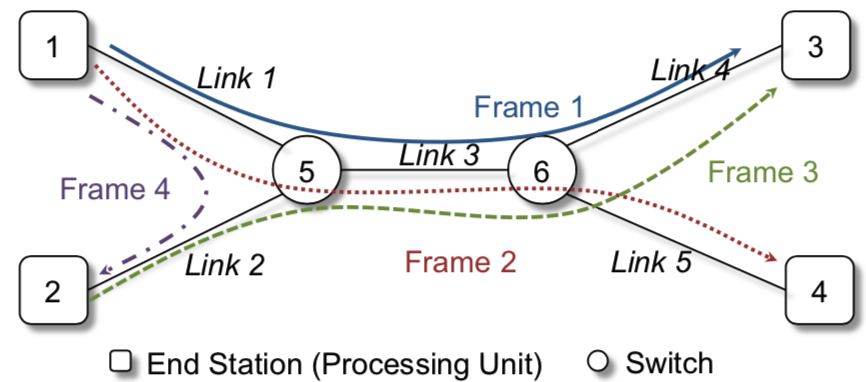
\includegraphics[width=0.5\textwidth]{network}
\label{fig:network}
\end{figure}

\subsection{MIP Formulation}
Zhang ~\cite{Zhang2018SynthesizingCA} formulates the application-level scheduling problem on a time-trigger, Ethernet-based switch network as an MIP problem. The tasks to be scheduled on the distributed system can be classified into application tasks that run on the end stations and communication tasks that should be scheduled on the Ethernet network. 

The first constraint on the MIP program formulation requires that application tasks are collision-free. The assumption for the distributed system is that each end station only consists of a single processor, so this constraint ensures that only one application task can be run on any end station at any given time stamp. The second constraint ensures that communication tasks are collision-free as well. At most one communication task can be transmitted on one direction of any link at any time stamp. 

Path dependency and data dependency are formulated as constraints as well. Path dependency for a communication task is formulated such that each frame has to be forwarded in the correct temporal order defined by its path to ensure that the message reaches the correct end station. Data dependency in application tasks requires application tasks and their corresponding communication tasks to be schedule in the correct temporal order. 

Constraints on response time and end-to-end latency on application tasks have also been exploited. Both the response time and the end-to-end latency are formulated as hard constraints, but adopting weakly hard constraints can provide looser constraints on response time, thus expanding the scope of schedulable task sets. Future work can be done on this direction.

Zhang ~\cite{Zhang2018SynthesizingCA} considered multiple objectives in this problem formulation. These objectives include response time and end-to-end latency in the average case and in the worst case, as well as certain timing requirements on specific tasks. The objective function, as a result, is a sum of each weighted sub-objective.



\section{Open Question} \label{rotation}

\subsection{Overview}
This section considers an open question: how to enhance the robustness of distributed embedded control systems utilizing the weakly hard model. The solution of this question can be applied to improving the security and robustness of automatic vehicles. A classical method to enhance the robustness of distributed system is to increase the redundancy of the system components so that single-point failure can be avoided. However, embedded control systems, e.g. control systems on automatic vehicles, have limited resources and therefore cannot afford a high level of redundancy. On the other hand, control systems can tolerant a certain level of occasional, bounded deadline misses as demonstrated in~\cite{liang2019security, maggio2020control, ramanathan1999overload, goswami2014relax, horssen2016performance, linsenmayer2017stabilization, pazzaglia2018beyond}. Therefore, we can utilize this property to optimize the assignments of application-level control tasks on processors. 

The approach is as follows: first, we analyze the deadline miss pattern for each control task in the m-K weakly hard model (Definition~\ref{def:missany}). Then, we map the control tasks to processors in a way that the tasks are rotating to a different processor in the next time stamp. Each time a processor encounters fatal errors and stops working, we adjust the mapping to fulfill the stability and control performance requirements for each control task, based on its deadline miss pattern. The mapping problem can be formulated as a MIP problem that optimizes the stability and control performance of the task set. Figure~\ref{fig:rotationmap} presents a model of two control tasks that are mapped onto two processor cores. 

\begin{figure}[h]
\caption{A model of systems with rotational control tasks mapping}
\centering
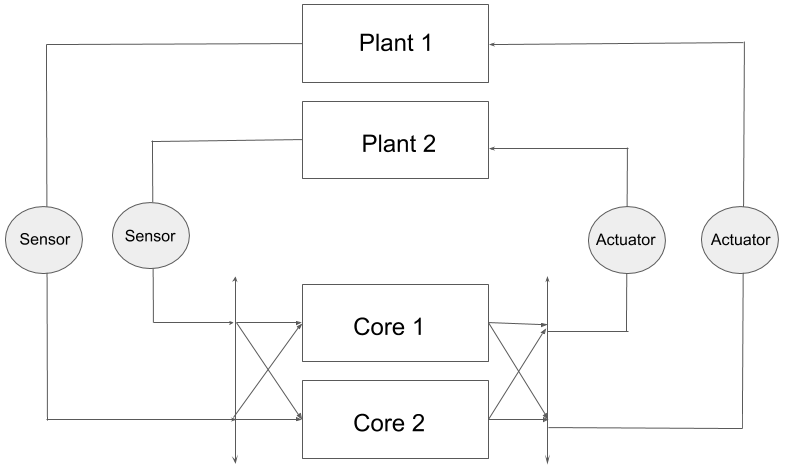
\includegraphics[width=0.5\textwidth]{rotationmap}
\label{fig:rotationmap}
\end{figure}

\subsection{Deadline Miss Pattern}
We consider the deadline miss pattern for each control task in the m-K weakly hard model (Definition~\ref{def:missany}). We assume that the system platform adopts a static-priority based, preemptive policy. A task set is defined as follows:
\begin{align*}
\tau = \{\tau_1, \tau_2, ..., \tau_n\}
\end{align*}
$\forall i \in {1, 2, ..., n}$, $\tau_i$ is a tuple of the following form:
\begin{align*}
\tau_i  = (c_{\tau_i}, d_{\tau_i}, t_{\tau_i}, p_{\tau_i})
\end{align*}
where $c_{\tau_i}$ is the worst-case execution time (WECT), $d_{\tau_i}$ is the deadline, $t_{\tau_i}$ is the period, and $p_{\tau_i}$ is the priority of $\tau_i$. 

We can use analysis technique proposed in~\cite{liang2019security, goswami2014relax} to analytically calculate an upper bound on the deadline miss pattern for each control task that ensures the stability of the task. 

\subsection{Objective Function}
We formulate the control tasks mapping problem as an MIP problem. The objective of this MIP formulation is to optimize the stability and control performance of the control tasks. To optimize the stability, we define a variable \textit{S} such that 
\begin{align*}
S &= \sum_{i=1}^n b_i \\
b_i &= \twopartdef {0} {\tau_i \: is \: stable} {1} {\tau_i \: is \: unstable}
\end{align*}
Here, \textit{$b_i$} is a binary decision variable that represents whether task $\tau_i$ is table or not. Then, by minimizing \textit{S}, we can have the maximum number of tasks that fulfill the stability requirement.

For control performance requirement, we can use the method described in Section ~\ref{stability and control performance}, as well as in ~\cite{liang2019security}, to describe the number of minimum required sample intervals needed to bring the system which is suffered from a disturbance back to the equilibrium state. We use \textit{H} to describe the control performance for all tasks. Thus, the objective function is:
\begin{align*}
minimize \;&\alpha\textit{S} + \beta\textit{H}
\end{align*}
where $\alpha$ and $\beta$ are predefined weights that are used to study the trade-off between two objectives.

\subsection{Constraints}
We now attempt to create constraints for the MIP formulation. The first type of constraints ensures that control tasks and communication tasks are collision-free, so that at any given time stamp, at most one control task will be running on any processor core, and at most one communication task will be transmitted on any communication bus. The formulation of a similar type of constraint is proposed in~\cite{Zhang2018SynthesizingCA}.

We then formulate constraints that encode the data dependency requirement for control tasks as well as path dependency requirement for communication tasks. Data dependency ensures that control tasks and their corresponding communication tasks are executed in the correct temporal order. Path dependency similarly impose temporal order to communication tasks so that they can be transmitted to the correct destination. Zhang ~\cite{Zhang2018SynthesizingCA} provides a general type of dependency constraint that can be of use in this solution.

Next, we encode timing constraints for the response time and end-to-end latency of each task. We use the method introduced in Section~\ref{weakly hard constraints formulation}~\cite{liang2019security} to set weakly hard constraints on tasks, and for those tasks not schedulable on the weakly hard model, hard constraints with a predefined maximum time requirement can be used.

Constraints are needed to ensure that the control tasks mapping will be changed from a time stamp to the next one. If we run the mapping algorithm every time stamp, so on each time stamp, we can encode the current mapping to be different from a predefined constant N which represents the number of past mappings in the most recent time stamps. However, the time to run the mapping algorithm on each time stamp is expensive in terms of time, and we will need to take this delay into our consideration. We can use heuristic search algorithm to aid the solving process of the MIP problem. An alternative approach is to analytically solve the MIP problem once with a default mapping to be in a round-robin manner. We predefine a temporal order of processor cores that each task by default is mapped to for each round. In this way, we don't need to run the MIP problem in run time and we do not need to have constraints about the order of processors each task is mapping to at every time stamp.


















\section{Conclusion} \label{conclusion}
This survey has reviewed recent works related to weakly hard constraints with an emphasis on its application to control systems. Various methods to compute and verify weakly-hard guarantees are studied. We focus on weakly hard model's applications to distributed embedded control systems such that the security and robustness of the systems are enhanced. We also study MIP formulation, an optimization technique common in the community of real-time systems. Lastly, we propose a new approach to leverage the weakly hard model to enhance the robustness of distributed embedded control systems in automatic vehicles.

\bibliographystyle{IEEEtran}
\bibliography{references}

\end{document}


